% ==============================================================================
% Section 4.3: Spatial Clustering (RQ2) — CORE SECTION
% ==============================================================================
\subsection{Spatial Clustering (RQ2)}
\label{sec:clustering}

\subsubsection{Global Spatial Autocorrelation}

Global Moran's $I$ confirms significant positive spatial autocorrelation across virtually the entire study period for all statuses.
Total and Not Located are significant in all 132 months (100\%); Located Alive in 127 of 132 (96.2\%); and Located Dead in 122 of 132 (92.4\%).
The five non-significant months for Located Alive and ten for Located Dead concentrate in the earliest months of the study period, when sparse counts limit statistical power (Figure~\ref{fig:morans}).

\begin{figure}[htbp]
  \centering
  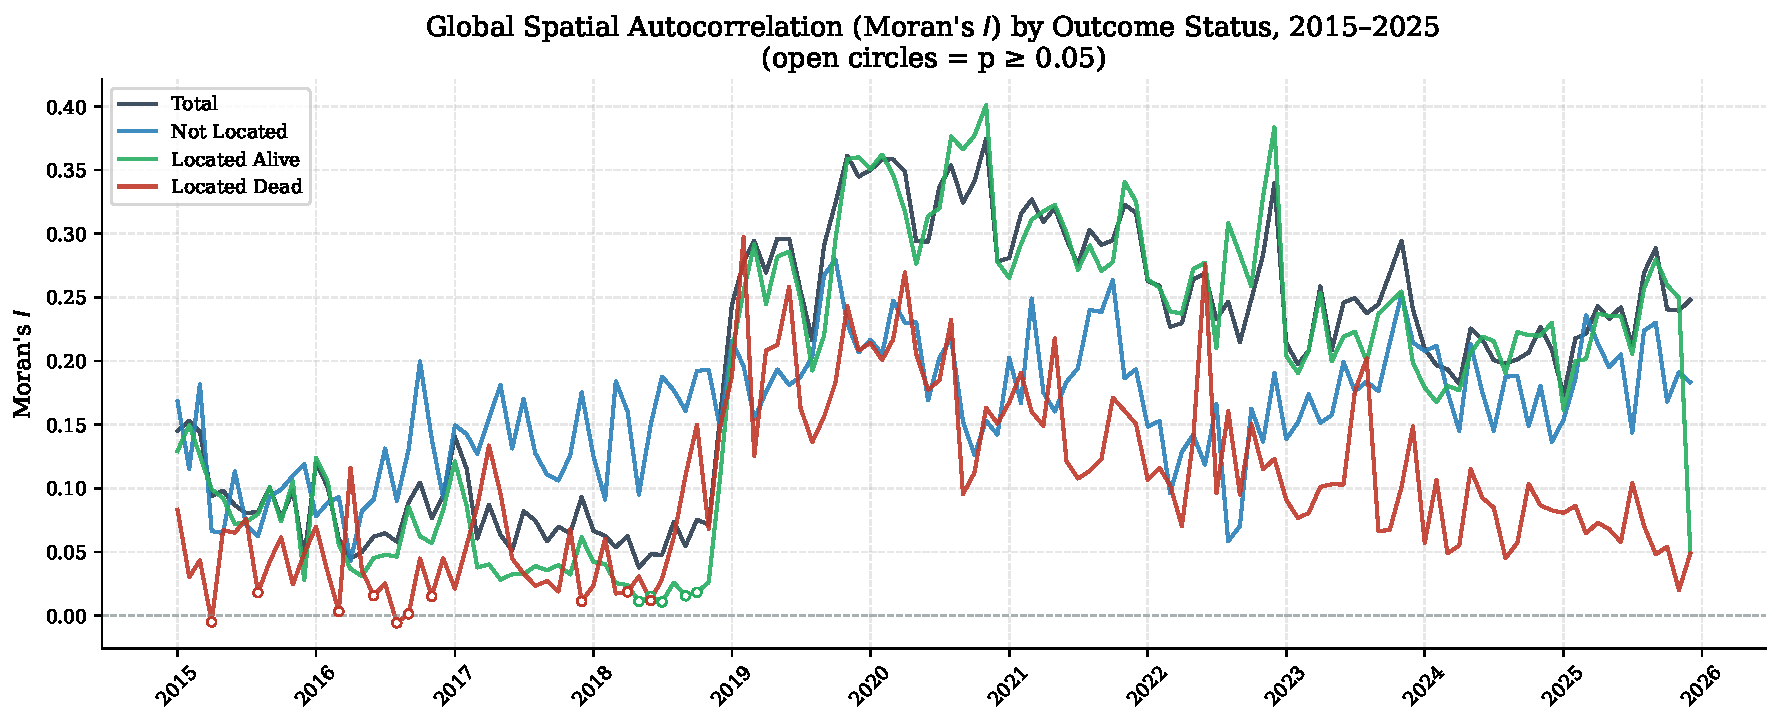
\includegraphics[width=\textwidth]{figures/fig3_morans_i_time_series.pdf}
  \caption{Global Moran's $I$ by outcome status, \studyperiod{}.
           Open circles indicate months with $p \geq 0.05$ (not statistically significant).}
  \label{fig:morans}
\end{figure}

The magnitude of spatial autocorrelation varies by status.
Total shows the highest mean $I$ (0.199, range: 0.038--0.374), followed by Located Alive (0.187, range: 0.011--0.401), Not Located (0.163, range: 0.043--0.280), and Located Dead (0.101, range: $-$0.006--0.298).
The lower values for Located Dead reflect the extreme sparsity of lethal-outcome cases across most of the country.

\subsubsection{LISA Classification}

Table~\ref{tab:lisa_counts} reports the LISA classification for \referencemonth{} (total sex).
Located Alive produces the most HH municipalities (110), followed by Total (106), Not Located (93), and Located Dead (35).
Located Dead stands out for its inverted LL--LH structure: only 7 LL municipalities but 105 LH municipalities, reflecting a pattern where most low-count municipalities are adjacent to at least one high-count neighbor.

\begin{tabular}{lrrrrrr}
  \toprule
  \textbf{Status} & \textbf{HH} & \textbf{LL} & \textbf{HL} & \textbf{LH} & \textbf{NS} & \textbf{Total} \\
  \midrule
  Total & 72 & 40 & 20 & 42 & 2,304 & 2,478 \\
  Not Located & 53 & 37 & 17 & 45 & 2,326 & 2,478 \\
  Located Alive & 52 & 45 & 10 & 56 & 2,315 & 2,478 \\
  Located Dead & 7 & 2,327 & 22 & 122 & 0 & 2,478 \\
  \bottomrule
  \multicolumn{7}{l}{\footnotesize LISA classification: Queen contiguity, 999 permutations, $\alpha=0.05$. Reference period: December 2025.} \\
  \multicolumn{7}{l}{\footnotesize HH = High-High, LL = Low-Low, HL = High-Low, LH = Low-High, NS = Not Significant.} \\
\end{tabular}

Figure~\ref{fig:lisa_latest} maps the LISA classification for all four statuses.
The geographic non-overlap is immediately visible.
Total and Located Alive HH clusters concentrate in Centro (Estado de M\'{e}xico, Puebla, CDMX corridor) with extensions into Norte.
Not Located HH clusters show a distinct Centro-dominated pattern with a secondary node in Norte.
Located Dead HH clusters are sparse and geographically restricted, with concentrations in Guanajuato and scattered municipalities in Tamaulipas and Jalisco.

\begin{figure}[htbp]
  \centering
  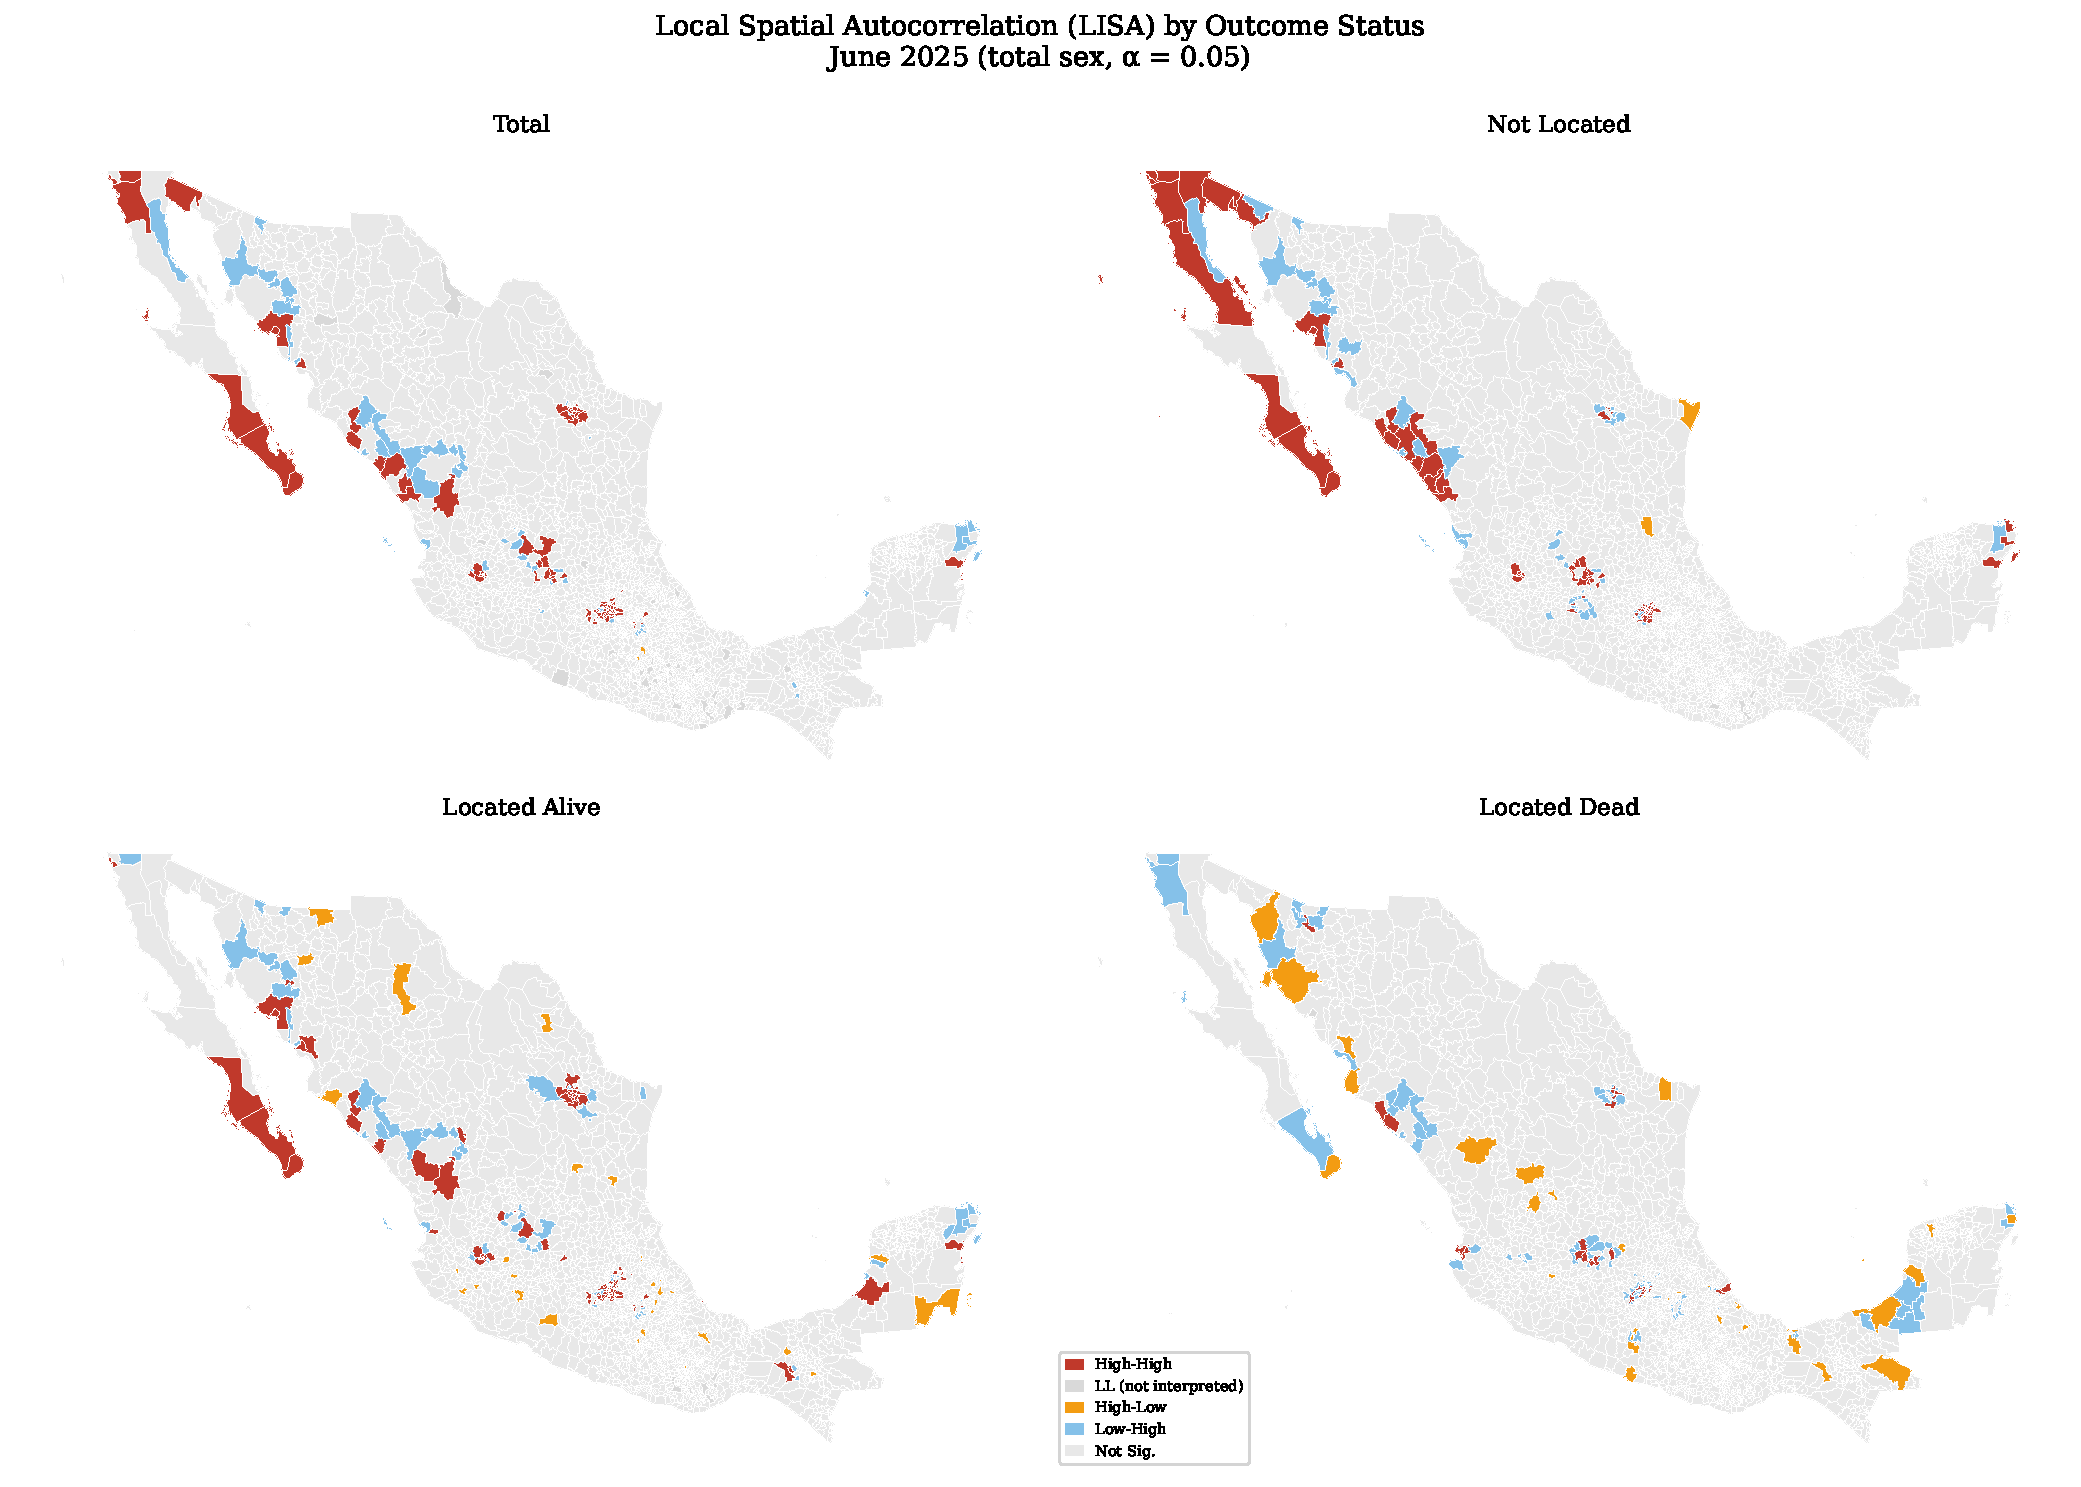
\includegraphics[width=\textwidth]{figures/fig4_lisa_maps_latest.pdf}
  \caption{LISA cluster maps by outcome status, \referencemonth{}.
           Red = High-High, grey = Low-Low (not interpreted; see Section~\ref{sec:lisa}),
           orange = High-Low, light blue = Low-High, white = Not Significant.
           Projection: EPSG:6372.}
  \label{fig:lisa_latest}
\end{figure}

\subsubsection{Non-Interchangeability: The Jaccard Evidence}

The paper's headline result is the quantitative demonstration that outcome statuses produce non-interchangeable spatial cluster geographies.
Table~\ref{tab:crosstab} reports pairwise Jaccard similarity coefficients (intersection over union of HH municipality sets) for \referencemonth{}.

\begin{tabular}{lrrrr}
  \toprule
  \textbf{} & \textbf{Total} & \textbf{Not Loc.} & \textbf{Located\,Alive} & \textbf{Located\,Dead} \\
  \midrule
  Total & \textbf{79} & 56 & 70 & 14 \\
  Not Loc. & 56 & \textbf{68} & 49 & 8 \\
  Located\,Alive & 70 & 49 & \textbf{91} & 12 \\
  Located\,Dead & 14 & 8 & 12 & \textbf{26} \\
  \bottomrule
  \multicolumn{5}{l}{\footnotesize Diagonal = total HH municipalities per status. Off-diagonal = pairwise intersection count.} \\
  \multicolumn{5}{l}{\footnotesize Reference period: June 2025. All counts use total sex LISA ($\alpha=0.05$).} \\
\end{tabular}

The Jaccard coefficients involving Located Dead are strikingly low: NL$\leftrightarrow$LD = 0.143 and LA$\leftrightarrow$LD = 0.151.
Only 14--15\% of the municipalities identified as hotspots for lethal outcomes overlap with hotspots for either Not Located or Located Alive cases.
The NL$\leftrightarrow$LA pair shows moderate overlap (0.381), suggesting some shared geography between active disappearances and recoveries.
The Total$\leftrightarrow$LA pair is highest (0.674), as expected given that Located Alive cases numerically dominate the Total series.

These results are stable across reference periods.
The Spearman rank correlation of local Moran's $I_i$ values between June 2024 and June 2025 ranges from 0.249 (Located Dead, total sex) to 0.607 (Total, total sex), confirming temporal stability in the underlying spatial structure (Appendix~\ref{app:robustness}).
The Jaccard pattern is also consistent across earlier cross-sections: in \bookendstart{}, NL$\leftrightarrow$LD Jaccard was 0.103 and LA$\leftrightarrow$LD was 0.000 (no overlap whatsoever between Located Alive and Located Dead hotspots).
